\chapter{Marketing da empresa}
\label{ch:identificador}

COMO FUNCIONA O MARKETING DA NOSSA EMPRESA

\section{O meio ambiente}
Nossa empresa promove uma ideia que além de pensar em melhorias nas entregas em delivery, pensamos também sobre o nosso meio ambiente, e o uso dos drones pode ajudar em alguns aspectos, observe:\\

\textbf{Redução de emissões de gases de efeito estufa:} As motos movidas a combustível fóssil contribuem para a poluição do ar, emitindo dióxido de carbono e outros poluentes. Os drones elétricos, por outro lado, não emitem gases de escapamento, o que reduz significativamente as emissões de carbono.\\

\textbf{Menor consumo de combustível:} Os drones consomem muito menos energia do que as motos para realizar entregas. Isso significa uma redução no consumo de combustível, que é geralmente derivado de fontes não renováveis, como o petróleo.\\

\textbf{Redução do tráfego nas estradas:} A substituição de motos por drones pode ajudar a diminuir o congestionamento nas estradas, já que os drones podem voar diretamente para o seu destino, evitando o trânsito terrestre. Menos veículos nas estradas também significam menos congestionamento e menos tempo perdido no tráfego.\\

\textbf{Promoção da inovação em energia limpa:} A transição para drones de entrega impulsiona o desenvolvimento e a adoção de tecnologias de energia limpa, como baterias mais eficientes e sistemas de propulsão elétrica. Isso pode ter efeitos positivos em outras áreas, incentivando o uso de energias renováveis e tecnologias mais limpas em diferentes setores\cite{Ifood2022}\cite{Ifood2021}. 

\section{Benefícios de se utilizar drones para entregas}

\textbf{Velocidade e eficiência:} Os drones podem voar diretamente para o seu destino, evitando congestionamentos de trânsito e rotas mais longas. Isso pode resultar em tempos de entrega significativamente mais curtos, especialmente em áreas urbanas.\\

\textbf{Acesso a áreas remotas:} Em regiões com infraestrutura de transporte subdesenvolvida ou em áreas remotas, os drones podem proporcionar uma maneira rápida e eficiente de realizar entregas, alcançando locais que seriam difíceis ou impossíveis de acessar por veículos terrestres.\\

\textbf{Redução de custos:} Embora os custos iniciais de implementação de sistemas de entrega por drones possam ser altos, a operação contínua tende a ser mais econômica do que os métodos tradicionais de entrega, especialmente a longo prazo. Isso inclui economias em combustível, manutenção de veículos e custos de mão de obra.\\

\textbf{Flexibilidade e escalabilidade:} Os drones podem ser facilmente adaptados para uma variedade de cargas e tamanhos de pacotes, desde pequenos itens até mercadorias maiores e mais pesadas. Além disso, a frota de drones pode ser facilmente escalada para atender à demanda sazonal ou flutuações de pedidos.\\

\textbf{Redução de emissões e impacto ambiental:} Como mencionado anteriormente, os drones elétricos não emitem poluentes atmosféricos durante o voo, o que contribui para a redução das emissões de gases de efeito estufa e a melhoria da qualidade do ar, comparado aos veículos terrestres movidos a combustíveis fósseis\cite{Ifood2022}\cite{Ifood2021}.

\section{Tráfego Pago}

Nossa empresa utiliza o método do tráfego pago para divulgação virtual do nosso produto. O tráfego pago nada mais é do que investir em plataformas de anúncios para divulgar seu site ou produto, fazendo assim com que seu produto seja mostrado mais frequentemente ao público, resultando em mais visibilidade e vendas.\\

Quais as vantagens do tráfego pago?\\

\textbf{Resultados imediatos:} Uma das maiores vantagens do tráfego pago é a capacidade de gerar resultados quase imediatos. Assim que uma campanha de publicidade é configurada e ativada, os anúncios podem começar a ser exibidos para o público-alvo, o que pode resultar em um aumento rápido no tráfego para o site ou oferta.\\

\textbf{Foco nas conversões:} o foco do tráfego pago é principalmente as conversões, empresas que pagam pelos anúncios, esperam que elas tenham um retorno significativo em vendas. As plataformas de publicidade online oferecem opções avançadas de segmentação que permitem direcionar os anúncios para públicos específicos com base em uma variedade de critérios, como idade, gênero, interesses, comportamento online, localização geográfica e muito mais. Isso ajuda a garantir que os anúncios sejam exibidos para as pessoas certas, aumentando a relevância e a eficácia da campanha.\\

\textbf{Flexibilidade de orçamento:} O tráfego pago oferece flexibilidade em termos de orçamento, permitindo que empresas de todos os tamanhos e setores participem. Os anunciantes podem definir um orçamento diário ou total para suas campanhas e ajustá-lo conforme necessário com base no desempenho e nos resultados obtidos.\\

\textbf{A estratégia direcionada por dados:} Pelo tráfego pago, é possível reunir informações sobre como os anúncios estão performando e quem é o público-alvo. Esse conhecimento possibilita aprimorar a estratégia continuamente, visando melhorar os resultados ao longo do tempo. Com base nessas análises, é viável adaptar a estratégia para aumentar o número de cliques, conversões e vendas\cite{Semrush2023}.

\section{Nossos drones}

Nós trabalhamos com três tipos de drones na nossa empresa, sendo eles:

\begin{figure} [!ht]
   {\centering
    \caption{DFH - 1}
    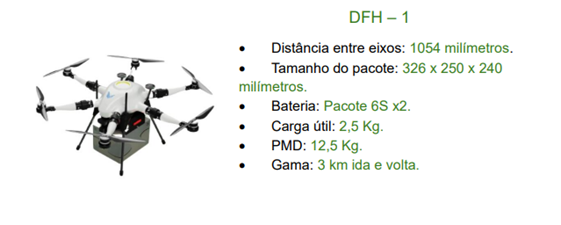
\includegraphics[width=0.9\linewidth]{figuras/drone dfh1.png}
    \label{fig:enter-label}
    \fonte{https://www.speedbird.aero/}
    }
\end{figure}

\begin{figure} [!ht]
    {\centering
    \caption{DFH - 2}
    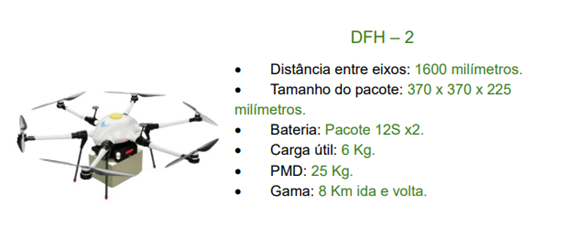
\includegraphics[width=0.9\linewidth]{figuras/drone dfh2.png}
    \label{fig:enter-label}
    \fonte{https://www.speedbird.aero/}
    }
\end{figure}

\begin{figure} [!ht]
 {   \centering
    \caption{DFH - 4}
    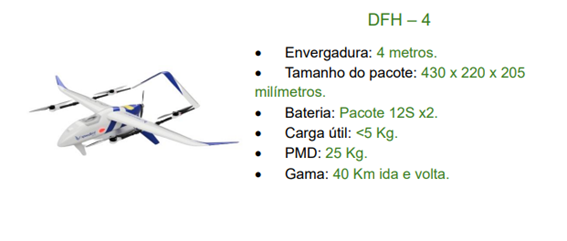
\includegraphics[width=0.9\linewidth]{figuras/drone dfh4.png}
    \label{fig:enter-label}
    \fonte{https://www.speedbird.aero/}
    }
\end{figure}

